%%----------------------------------------------------------------------------
%% Presentatie HoGent Bedrijf en Organisatie
%%----------------------------------------------------------------------------
%% Auteur: Bert Van Vreckem [bert.vanvreckem@hogent.be]

\documentclass{beamer}

%==============================================================================
% Aanloop
%==============================================================================

%---------- Packages ----------------------------------------------------------
\usepackage{etex}
\usepackage{graphicx,multicol}
\usepackage{comment,enumerate,hyperref}
\usepackage{amsmath,amsfonts,amssymb}
\usepackage{tikz}
\usepackage[dutch]{babel}
\usepackage[utf8]{inputenc}
\usepackage{multirow}
\usepackage{eurosym}
\usepackage{listings}
\usepackage[T1]{fontenc}
\usepackage{lmodern}
\usepackage{textcomp}
\usepackage{framed}
\usepackage{wrapfig}
\usepackage{pgf-pie}
\usepackage{pgfplots}
\usepackage{booktabs}
\usepackage{pgfplotstable}
\usepackage{changepage}
\usepackage{pst-plot,pst-func}

%---------- Configuratie ------------------------------------------------------

\usetikzlibrary{arrows,shapes,backgrounds,positioning,shadows}
\usetikzlibrary{pgfplots.statistics}
\newif\ifprivate
\privatetrue


\usetheme{hogent}
\setbeameroption{show notes}

%---------- Commando-definities -----------------------------------------------

\newcommand{\tabitem}{~~\llap{\textbullet}~~}
\renewcommand{\arraystretch}{1.2}

%---------- Info over de presentatie ------------------------------------------

\title[Intro]{Onderzoekstechnieken\\Tijdreeksen}
\author{Anita Bernard, Jens Buysse, Bert {Van Vreckem}}
\date{AJ 2016-2017}

%==============================================================================
% Inhoud presentatie
%==============================================================================

\begin{document}

%---------- Front matter ------------------------------------------------------

% Dia met het HoGent logo
\HoGentLogo

% Titeldia met faculteitslogo
\titleframe

%---------- Inhoud ------------------------------------------------------------

\begin{frame}
  \frametitle{What's on the menu today?}

  \tableofcontents
\end{frame}

\section{Tijdreeksen en voorspellingen}

\begin{frame}
  \frametitle{Tijdreeksen en voorspellingen}

  \brightbox{Een tijdreeks is een opeenvolging van observaties van een variabele in functie van de tijd}

  Een tijdreeks is een stochastisch proces. Voorbeelden:

  \begin{itemize}
    \item Maandelijkse vraag naar melk
    \item Jaarlijkse instroom van ``generatiestudenten'' aan de hogeschool
    \item Prijs van een aandeel of obligatie op de beurs (van uur tot uur, per dag, \dots)
    \item Aantal HTTP requests per seconde op een website
    \item Evolutie schijfgebruik op een backup-server
  \end{itemize}
\end{frame}

\begin{frame}
  \frametitle{Tijdreeksen en voorspellingen}

  Tijdreeksen zijn een belangrijk onderdeel van onderzoek omdat ze vaak de \textbf{basis} vormen voor beslissingsmodellen en voorspellingen.

  \begin{itemize}
    \item algemene ontwikkeling van toekomstplannen (investeringen, capaciteit \dots)
    \item plannen van budgettering om tekortkomingen te vermijden (operationeel budget, marketing budget \dots)
    \item ondersteuning van financi\"ele objectieven
    \item onzekerheid vermijden
  \end{itemize}
\end{frame}

\begin{frame}
  \frametitle{Tijdreeksen en voorspellingen}

  Tijdreeksen zijn een \textbf{statistisch} probleem: observaties variëren in functie van de tijd

  \begin{figure}
    \centering
    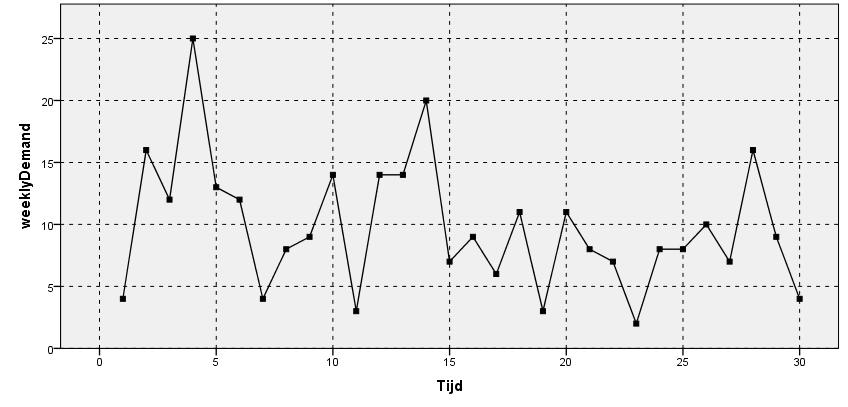
\includegraphics[width=\textwidth]{img/tijdreeks11}
    \caption{Tijdreeks voor de wekelijkse vraag voor een bepaald product}
  \end{figure}
\end{frame}

\section{Tijdreeksmodellen}

\subsection{Wiskundig model}

\begin{frame}
  \frametitle{Wiskundig model tijdreeks}

  Het eenvoudigste model:

  \begin{itemize}
    \item Constante $b$
    \item Variaties rond $b$ bepaald door willekeurige variabele $\varepsilon_{t}$
  \end{itemize}

  \begin{equation}
    X_{t} = b + \varepsilon_{t}
    \label{eq:tijdreeks-constante}
  \end{equation}

  \begin{itemize}
    \item $X_{t}$: stochastische variabele voor de tijdreeks, op tijdstip $t$
    \item $x_{t}$: \emph{observatie} op tijdstip $t$ (dus gekend!)
    \item $\varepsilon_{t}$ noemt men de \emph{storing} (Eng: \emph{noise}). We veronderstellen $\varepsilon_{t} \sim Nor(\mu = 0; \sigma)$
  \end{itemize}
\end{frame}

\begin{frame}
  \frametitle{Wiskundig model tijdreeks}

  We kunnen er ook van uit gaan dat er een lineair verband is:

  \begin{equation}
    X_{t} = b_{0} + b_{1} \times t + \varepsilon_{t}
    \label{eq:tijdreeks-lineair}
  \end{equation}

  Vergelijkingen~\ref{eq:tijdreeks-constante} en \ref{eq:tijdreeks-lineair} zijn speciale gevallen van het \emph{polynomiale} geval:

  \begin{equation}
    X_{t} = b_{0} + b_{1} t + b_{2} t^{2} + \dots + b_{n} t^{n} + \varepsilon_{t}
    \label{eq:tijdreeks-polynomiaal}
  \end{equation}
\end{frame}

\subsection{Algemeen}

\begin{frame}
  \frametitle{Algemene uitdrukking tijdreeks}

  \begin{equation}
    X_{t} = f(b_{0}, b_{1}, b_{2}, \dots , b_{n}, t) + \varepsilon_{t}
    \label{eq:tijdreeks-algemeen}
  \end{equation}

  We gaan verder uit van deze veronderstellingen:

  \begin{itemize}
    \item We beschouwen twee componenten van variabiliteit:
      \begin{itemize}
        \item het gemiddelde van de voorspellingen verandert in de tijd
        \item de variaties ten opzichte van dit gemiddelde variëren willekeurig
      \end{itemize}
    \item De variatie van de residuen van het model ($X_t - x_t$) is constant in de tijd (\emph{homeoscedastisch})
  \end{itemize}
\end{frame}

\subsection{Schatten van de parameters}

\begin{frame}
  \frametitle{Schatten van de parameters}

  \emph{Voorspellingen} maken aan de hand van tijdreeksmodel:

  \begin{enumerate}
    \item selecteer het meest passende model
    \item schatting voor parameters $b_i (i: 1, \dots, n)$ a.h.v.~observaties
  \end{enumerate}

  Deze schattingen $\widehat{b_i}$ zijn dan zodanig dat ze de geobserveerde waarden zo goed mogelijk benaderen.
\end{frame}

\begin{frame}
  \frametitle{Voorbeeld}

  \begin{table}[t]
    \centering
    \begin{tabular}{|l|l|l|l|l|l|l|l|l|l|}
      \hline
      4 & 16 & 12 & 25 & 13 & 12 & 4 & 8  & 9 & 14 \\ \hline
      3 & 14 & 14 & 20 & 7  & 9  & 6 & 11 & 3 & 11 \\ \hline
      8 & 7  & 2  & 8  & 8  & 10 & 7 & 16 & 9 & 4  \\ \hline
    \end{tabular}
    \label{tab:data}
    \caption{Tijdreeks voor de wekelijkse vraag voor een product}
  \end{table}

  \begin{figure}
    \centering
    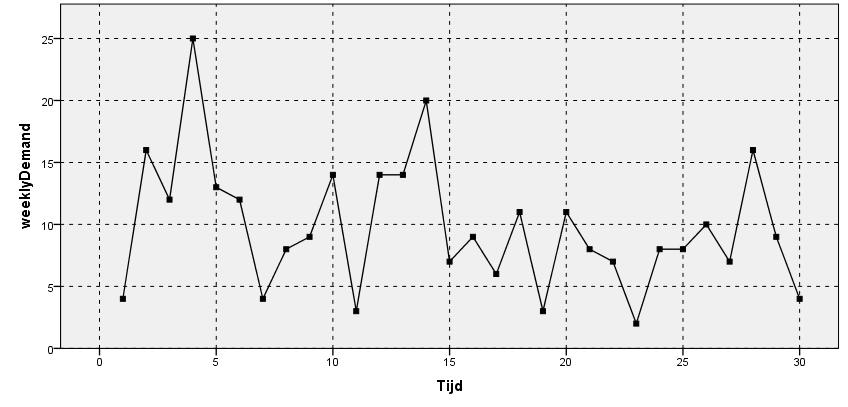
\includegraphics[width=.7\textwidth]{img/tijdreeks11}
  \end{figure}
\end{frame}

\begin{frame}
  \frametitle{Voorbeeld: Parameterschatting}

  \begin{itemize}
    \item We kiezen het constante model uit vergelijking~\ref{eq:tijdreeks-constante}
    \item Als schatter voor $b$ kiezen we het gemiddelde van de eerste 20 observaties:

      \[ \widehat{b} = \frac{1}{20} \sum_{t = 1}^{20} x_{t}= 10.75 \]

  \end{itemize}

  \centering
  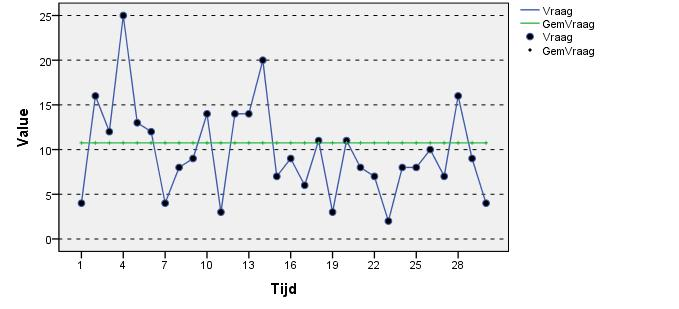
\includegraphics[width=.7\textwidth]{img/tijdreeks21.jpg}
\end{frame}

\begin{frame}
  \frametitle{Voorbeeld: parameterschatting}

  Je kiest zelf welke observaties je gebruikt voor het bepalen van $\widehat{b}$, bv.:

  \begin{itemize}
    \item $\widehat{b} = \frac{1}{10} \sum_{10}^{20} x_{t} = 10.18$
    \item $\widehat{b} = \frac{1}{5} \sum_{15}^{20} x_{t} = 7.83$
  \end{itemize}

\end{frame}

\section{Voortschrijdend gemiddelde}

\subsection{Eenvoudig voortschrijdend gemiddelde}

\begin{frame}
  \frametitle{Voortschrijdend gemiddelde}

  \brightbox{Het eenvoudig voortschrijdend gemiddelde is een reeks \emph{gemiddelden} van de laatste $m$ observaties}

  \begin{itemize}
    \item Eng.: \emph{Simple Moving Average} (SMA)
    \item Verbergen korte-termijn fluctuaties en tonen lange-termijn trends
    \item $m$ is het tijdbereik (time range), en is de parameter van deze methode
  \end{itemize}

  \begin{equation}
    SMA(t) = \sum_{i=k}^{t} \frac{x_{i}}{m}
    \label{eq:movingAverage}
  \end{equation}

  met $k = t - m + 1$.
\end{frame}

\begin{frame}
  \frametitle{Voorbeeld: ``Golden cross''}

  Moving Averages worden gebruikt in \emph{technische analyse} van aandelenkoersen om trends te ontdekken:

  \begin{center}
    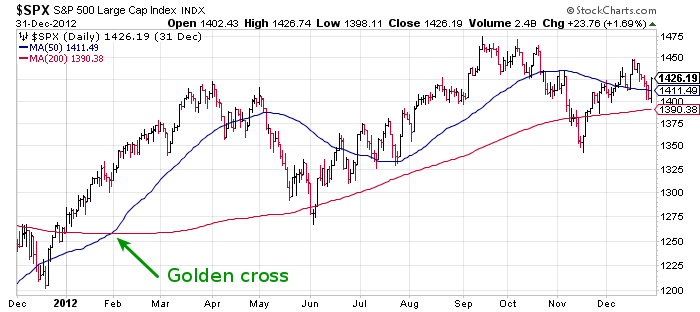
\includegraphics[width=\textwidth]{img/tijdreeks-golden-cross}
  \end{center}
\end{frame}

\note{%
  Deze grafiek is de koers van de S\&P500 index (vergelijk met onze Bel-20) voor december 2011 tot eind 2012. In de grafiek worden de SMA's van de prijs bij sluitingstijd van de 50 en 200 laatste beursdagen gegeven (notatie: MA(50) en MA(200)). Wanneer de markt in een dalende trend zit (``\textbf{bear market}''), ligt de MA(200) boven MA(50) (zie linkse deel van de tekening).

  In februari 2012 ging MA(50) boven de MA(200), een verschijnsel dat ``\textbf{the golden cross}'' genoemd wordt. De stijging van de index was al enkele maanden eerder ingezet, maar de MA's reageren uiteraard trager.

  Een \emph{golden cross} is een indicator dat de markt (of een specifiek aandeel) in een lange-termijn stijgende trend zit (``\textbf{bull market}''). In dit geval duurt deze trend nog voort tot vandaag (voorjaar 2015).

  De MA(200)-lijn wordt dan beschouwd als ``steunpunt'', d.w.z.~een ondergrens voor het koerscijfer. Aan deze prijs is het aandeel heel interessant, stijgt de vraag en wordt de koers terug omhoog getrokken.

}

\begin{frame}
  \begin{table}
    \begin{tabular}{|llllllllll|}
      \hline
      ~       & 11   & 12   & 13   & 14   & 15   & 16   & 17   & 18   & 19   \\
      $x_{t}$ & 3    & 14   & 14   & 20   & 7    & 9    & 6    & 11   & 3    \\
      $X_{t}$ & 11.7 & 11.6 & 11.4 & 11.6 & 11.1 & 10.5 & 10.2 & 10.4 & 10.7 \\
      $e$     & -8.7 & 2.4  & 2.6  & 8.4  & -4.1 & -1.5 & -4.2 & 0.6  & -7.7 \\ \hline
    \end{tabular}
    \caption{Voorspellingsfout voor een moving average $m = 10$}
    \label{tab:error}
\end{table}

Een methode om de voorspelling te meten is het gemiddelde van de deviaties ($MAD$).

\begin{equation}
  MAD = \frac{1}{n} \sum_{1}^{n} \left| e_{i} \right|
\label{eq:MAD}
\end{equation}

Je kan ook de variantie ervan bepalen:

\begin{equation}
  s^{2}_{e} = \frac{1}{m} \sum_{1}^{n} (e_{i} - \overline{e})^{2}
\label{eq:varError}
\end{equation}
\end{frame}

\subsection{Gewogen voortschrijdend gemiddelde}

\begin{frame}
  \frametitle{Gewogen voortschrijdend gemiddelde}

  \begin{itemize}
    \item Bij $SMA$ zijn de gewichten van de observaties gelijk
    \item Bij gewogen voortschrijdend gemiddelde (weighted moving average, $WMA$) wegen recentere observaties meer door
    \item Een specifieke vorm hiervan is exponentiële afvlakking (exponential smoothing) of het \emph{exponentieel voortschrijdend gemiddelde} ($EMA$):
      \begin{equation}
        EMA(t) = \alpha x_{t-1} + (1-\alpha) EMA(t-1)
        \label{eq:singleExpSmooting}
      \end{equation}

      met $\alpha$ de smoothing constante ($0 < \alpha < 1$), en $t \geq 3$
  \end{itemize}
\end{frame}

\begin{frame}
  \frametitle{Exponentiële afvlakking}

  Formule~\ref{eq:singleExpSmooting} geldt enkel vanaf $t=3$. Het bepalen van $EMA(2)$ is een belangrijke parameter.

  Er zijn verschillende keuzes:

  \begin{itemize}
    \item $EMA(2) = x_1$
    \item $EMA(2) = \frac{1}{m} \sum_{i=1}^{m} x_i$ (dus gemiddelde van de eerste $m$ observaties)
    \item $EMA(2)$ gelijk stellen aan een bepaald objectief
    \item \ldots
  \end{itemize}
\end{frame}

\begin{frame}
  \frametitle{Waarom ``\emph{exponentieel}''?}

  \begin{eqnarray*}
    EMA(t) & = & \alpha x_{t-1} + (1-\alpha) EMA(t-1)                                           \\
           & = & \alpha x_{t-1} + (1-\alpha)\left[\alpha x_{t-2} + (1-\alpha)EMA(t - 2)\right]  \\
           & = & \alpha x_{t-1} + \alpha (1-\alpha)x_{t-2} + (1-\alpha)^{2} EMA(t - 2)          \\
           &   & \text{of algemeen gesteld:} \\
           & = & \alpha \sum_{i=1}^{t-2}(1-\alpha)^{i-1}x_{t-i} + (1-\alpha)^{t-2} EMA(2), t \geq 2
  \end{eqnarray*}

  M.a.w.~oudere observaties krijgen een exponentieel kleiner gewicht.
\end{frame}

\begin{frame}
  \frametitle{Exponentiële afvlakking}

  \begin{table}
    \centering
    \begin{tabular}{l|llll}
      $\alpha$ & $(1-\alpha)$ & $(1-\alpha)^{2}$ & $(1-\alpha)^{3}$ & $(1-\alpha)^{4}$ \\ \hline
      0.9   & 0.1       & 0.01             & 0.001                      & 0.0001           \\
      0.5   & 0.5       & 0.25             & 0.125                      & 0.062            \\
      0.1   & 0.9       & 0.81             & 0.729                      & 0.6561           \\
    \end{tabular}
    \caption{Waarden voor $\alpha$ en $(1-\alpha)^{n}$}
    \label{tab:alpha}
  \end{table}
  De snelheid waarmee de oude observaties ''vergeten`` worden hang af van $\alpha$. Met een $\alpha$ dicht bij 1 vergeet je snel, terwijl een $\alpha$ dicht bij nul ervoor zorgt dat dat vergeten minder snel gaat
\end{frame}


\begin{frame}
  \frametitle{Voorbeeld}
  \begin{figure}[htbp]
    \centering
    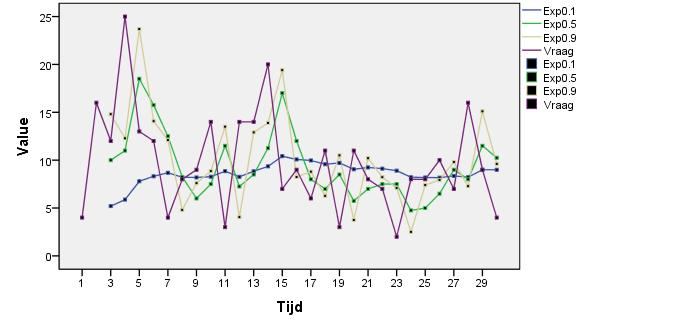
\includegraphics[width=\textwidth]{img/tijdreeks51}
    \caption{Enkelvoudige exponentiële afvlakking met $\alpha=0.1 , 0.5, 0.9$}
    \label{fig:tijdreeks51}
  \end{figure}
\end{frame}

\subsection{Dubbele exponenti\"ele afvlakking}

\begin{frame}
  \frametitle{Dubbele exponenti\"ele afvlakking}

  Enkelvoudige afvlakking werkt niet goed als er een trend in de data zit

  \begin{figure}
    \centering
    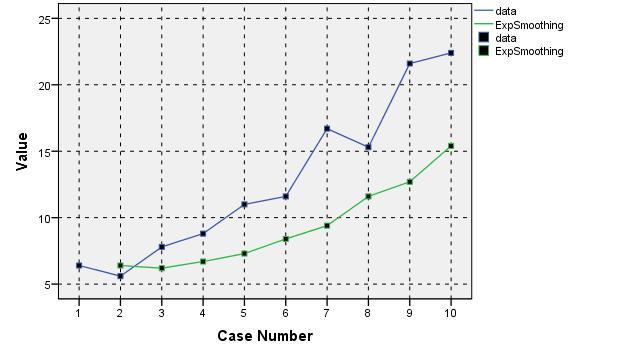
\includegraphics[width=.7\textwidth]{img/tijdreeks61}
    \caption{Exponenti\"ele afvlakking bij een trend: de fouten worden steeds groter}
    \label{fig:tijdreeks61}
  \end{figure}

\end{frame}


\begin{frame}
  \frametitle{Dubbele exponentiële afvlakking}

  We voeren een extra term in om de trend te modelleren. We noteren $s_t$ voor de afgevlakte waarde, en $b_t$ voor de schatting van de trend op tijdstip $t > 1$:

\begin{eqnarray}
	X_{t} = \alpha x_{t} + (1-\alpha)(X_{t-1} + b_{t-1}) & 0 \leq \alpha \leq 1 \\
	b_{t} = \gamma(X_{t}-X_{t-1}) + (1-\gamma)b_{t-1} & 0 \leq \gamma \leq 1 
\label{eq:doubleSmoothing}
\end{eqnarray}

  met $0 < \alpha < 1$ en $0 < \gamma < 1$
	
	
	\begin{itemize}
		\item De $ b_{t-1}$ in de eerste vergelijking zorgt voor het volgen van de trend
		\item $X_{t}-X_{t-1}$ is postief of negatief en zorgt ervoor dat de trend gegenereerd wordt
	\end{itemize}
\end{frame}

\begin{frame}
  \frametitle{Dubbele exponentiële afvlakking}
  Er bestaan opnieuw verschillende alternatieven om de initiële waarden te kiezen:

\begin{eqnarray}
	X_{1} = x_{1} \\
	b_{1} = x_{2} - x_{1} \\
	b_{1} = \frac{1}{3}\left[ (x_{2} - x_{1}) + (x_{1} - x_{2}) + (x_{4} - x_{3}) \right]\\
	b_{1} = \frac{x_{n} - x_{1}}{n-1} \\
\end{eqnarray}

\end{frame}

\subsubsection{Voorspellen}

\begin{frame}
  \frametitle{Voorspellen}

  Om een voorspelling $F(t+1)$ te maken voor tijdstip $t+1$ gebruiken we:

  \[ F(t+1) = s_t + b_t \]

  of algemeen voor tijdstip $t+m$:

  \[ F(t+m) = s_t + m b_t \]
\end{frame}

\begin{frame}
  \begin{figure}
    \centering
    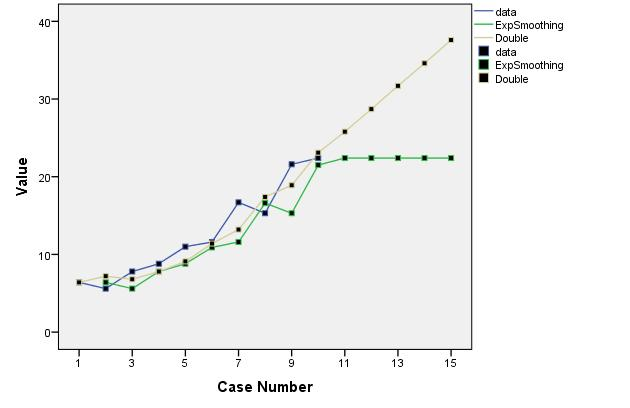
\includegraphics[width=\textwidth]{img/tijdreeks71}
    \caption{Enkelvoudige en dubbele afvlakking}
    \label{fig:tijdreeks71}
  \end{figure}
\end{frame}

\subsection{Driedubbele exponentiële afvlakking}

\begin{frame}
  \frametitle{Driedubbele exponentiële afvlakking}

  of methode van Holt-Winters. Deze houdt rekening met seizoenaliteit in de data. We noteren:

  \begin{itemize}
    \item $L$: lengte van de seizoenale cyclus (aantal tijdseenheden)
    \item $c_t$: term die de seizoenale variaties modelleert
    \item $\gamma$: smoothing factor voor de seizoenale variatie
  \end{itemize}

\begin{eqnarray*}
	X_{t} = \alpha \frac{x_{t}}{c_{t-L}} + (1-\alpha) (X_{t-1} + b_{t-1}) & \textnormal{Smoothing}\\
	b_{t} = \gamma (X_{t} - X_{t-1}) + (1-\gamma)b_{t-1} & \textnormal{Trend smoothing} \\
	c_{t} = \beta \frac{x_{t}}{X_{t}} + (1-\beta)c_{t-L} & \textnormal{Seasonal smoothing} \\
\label{eq:HoltWinters}
\end{eqnarray*}

\end{frame}

\begin{frame}
  \frametitle{Driedubbele exponentiële afvlakking}

  Voorspelling op tijdstip $t + m$:

  \[ F_{t+m} = (X_{t} + mb_{t})c_{t-L+m}  \textnormal{Voorspelling}\]

  Voor een implementatie in Java, zie \url{https://github.com/bertvv/wintersmethod}
\end{frame}

\begin{frame}
  \frametitle{Voorbeeld: voorspel verkoopscijfers}

  \centering
  \begin{tikzpicture}
    \begin{axis}[
        title=Geobserveerde Verkoopscijfers,
        xlabel=Weekdag,
        ylabel=SKUs,
      ]
      \addplot table [x index=0, y index=1, col sep=comma] {data/shoestore-sales.dat};
    \end{axis}
  \end{tikzpicture}
\end{frame}

\begin{frame}
  \frametitle{Voorbeeld}

  Keuze startwaarden:

  \begin{itemize}
    \item smoothing factors: $\alpha = 0.8, \beta = 0.8, \gamma = 0.3$
    \item $s_0 = 5849$, $b_0 = 123.3$
    \item $L = 7$ (dus wekelijks terugkerend), dan hebben we ook 7 waarden nodig om $c_t$ te initialiseren (zie tabel)
  \end{itemize}

  \begin{table}
    \centering
    \begin{tabular}{l|l|l|l}
      ma ($c_0$) & di ($c_1$) & wo ($c_2$) & do ($c_3$)  \\
      1.245693 & 1.115265 & 1.088853 & 1.135378 \\
      \hline \hline
      vr ($c_4$)  & za ($c_5$)  & zo ($c_6$)  & \\
      1.178552 & 1.229739 & 0.006520 &
    \end{tabular}
    \caption{Startwaarden voor $c_t$}
    \label{tab:winters-init-c}
  \end{table}
\end{frame}

\begin{frame}
  \frametitle{Voorbeeld: voorspelling}


  \begin{center}
  \begin{tikzpicture}
    \begin{axis}[
        scale=.8,
        title=Verkoopscijfers,
        xlabel=Weekdag,
        ylabel=SKUs,
        unbounded coords=jump,
        legend to name=bottomlegend,
      ]
      \addplot table [x index=0, y index=1, col sep=comma] {data/shoestore-sales.dat};
      \addlegendentry{Geobserveerd}
      \addplot table [x index=0, y index=2, col sep=comma] {data/shoestore-sales.dat};
      \addlegendentry{Voorspeld}
    \end{axis}
  \end{tikzpicture}

  \ref{bottomlegend}
\end{center}

\end{frame}


\end{document}

